% LaTeX Template for Project Report, Version 2.0
% (Abstracted from a Major Project Report at CSED, NIT Calicut but can be
% modified easily to use for other reports also.)
%
% Released under Creative Commons Attribution license (CC-BY)
% Info: http://creativecommons.org/licenses/by/3.0/
%
% Created by: Kartik Singhal
% BTech CSE Batch of 2009-13
% NIT Calicut
% Contact Info: kartiksinghal@gmail.com
%
% It is advisable to learn the basics of LaTeX before using this template.
% A good resource to start with is http://en.wikibooks.org/wiki/LaTeX/
%
% All template fields are marked with a pair of angular brackets e.g. <title here>
% except for the ones defining citation names in ref.tex.
%
% Empty space after chapter/section/subsection titles can be used to insert text.
%
% Just compile this file using pdflatex after making all required changes.

\documentclass[11pt,letter]{report}
\usepackage[pdftex]{graphicx} %for embedding images
\usepackage{url} %for proper url entries
\usepackage[bookmarks, colorlinks=false, pdfborder={0 0 0}, pdftitle={<pdf title here>}, pdfauthor={<author's name here>}, pdfsubject={<subject here>}, pdfkeywords={<keywords here>}]{hyperref} %for creating links in the pdf version and other additional pdf attributes, no effect on the printed document
%\usepackage[final]{pdfpages} %for embedding another pdf, remove if not required

\begin{document}
\renewcommand\bibname{References} %Renames "Bibliography" to "References" on ref page

%include other pages
\begin{titlepage}

\begin{center}

\textup{\small {\bf CSCI-2950U} \\ Project Report}\\[0.5in]

% Title
\Large \textbf {End-to-end Tracing for Serverless Applications}\\[1in]

       \small \emph{Submitted in partial fulfillment of\\
        the requirements for the award of the degree of}
        \vspace{.4in}

       {\bf Master of Science \\in\\ Computer Science}\\[0.6in]

% Submitted by
\normalsize Submitted by \\

\Large Kartik Singhal \\

\normalsize kartik@cs.brown.edu


\vfill

% Bottom of the page

\includegraphics[width=0.45\textwidth]{./brown_cs_logo}\\[0.1in]
\Large{Department of Computer Science}\\
\normalsize
\textsc{Brown University}\\
Providence, Rhode Island, USA -- 02912 \\
\vspace{0.2cm}
Spring 2017

\end{center}

\end{titlepage}

\vspace{2in}
\begin{abstract}

From bare metal, to virtual machines, to containers and now to serverless, the cloud computing industry is making it easier and easier for developers to focus on writing code and not worry about how and where to deploy it. With this ease of use comes the problem of lack of visibility into the software stack, which is a critical need when things go wrong in production. We study the problem of tracing and instrumentation in distributed environments and present ongoing work on instrumenting an open source serverless framework, \emph{OpenWhisk}, using one of the most flexible and pervasive tracing platforms, \emph{Brown University Tracing Framework}.

\end{abstract}


\pagenumbering{roman} %numbering before main content starts
\tableofcontents
\listoffigures

\newpage
\pagenumbering{arabic} %reset numbering to normal for the main content

\input{./prob-definition.tex} %objective changed to problem definition
\chapter{Introduction}

\section{Background}

\subsection{Serverless Computing or Function as a Service (FaaS)}
Serverless computing is a relatively recent cloud computing model in which a cloud provider fully manages execution of user specified functions without the user having to worry about provisioning containers (and earlier virtual machines (VM)) for their use. One of the primary benefits apart from abstration is in terms of cost as the providers usually only charge for the resources used during the execution of a request instead of hourly or per-VM billing.

The programming model is that the unit of execution is a funtion which can be invoked through an HTTP API. A more general model of event-driven programming is also supported in that one can schedule actions that can trigger periodically or by explicit request through HTTP.

Most major cloud service providers have introduced their own serverless offerings, such as Amazon's AWS Lambda, Google's Cloud Functions, IBM's OpenWhisk (or Apache OpenWhisk\cite{web:wsk}), and Microsoft's Azure Functions.

However, debugging or tracing one's application in this architecture remains a difficulty as users have little to no visibility into the underlying software stack. Even if one can replicate an open source offering such as OpenWhisk in their local environment, tracing across diverse system components in a distributed setting is a difficult problem as we discuss in the next section.

\subsection{Why is Tracing Distributed Systems hard?}


\begin{itemize}
  \item Towards a Tracing Plane for Distributed Systems\cite{Fonseca16}
  \item A Layered Architecture for Distributed System Instrumentation\cite{Mace17}
  \item X-trace: A Pervasive Network Tracing Framework\cite{Fonseca:2007:XPN:1973430.1973450}
  \item Pivot Tracing: Dynamic Causal Monitoring for Distributed Systems\cite{Mace:2015:PTD:2815400.2815415}
  \item End-to-End Tracing: Adoption and Use Cases\cite{mace2017survey}
  \item Conflict-free Replicated Data Types\cite{Shapiro:2011:CRD:2050613.2050642}
  \item A comprehensive study of Convergent and Commutative Replicated Data Types\cite{shapiro:inria-00555588}
  \item Apache OpenWhisk\cite{web:wsk}
  \item Brown Tracing Framework\cite{web:btf}
  \item Zipkin
\end{itemize}

\section{Motivation}
 %literature survey included in this
\chapter{Work Done}
We started out by trying to find a good application to instrument using Tracing Plane abstractions and investigated a couple of distributed concurrent programming frameworks, namely Akka and Finagle. But we soon realized that a typical distributed system used in production is built using a lot of different components and focusing on homogeneous framworks such as Finagle will not reveal the intricacies that we would like to learn about in instrumenting using tracing plane. We ultimately decided on OpenWhisk as it both seemed like a typical distributed system and seemed well supported by the community.

\section{Apache OpenWhisk}
\begin{figure}[htb]
\centering
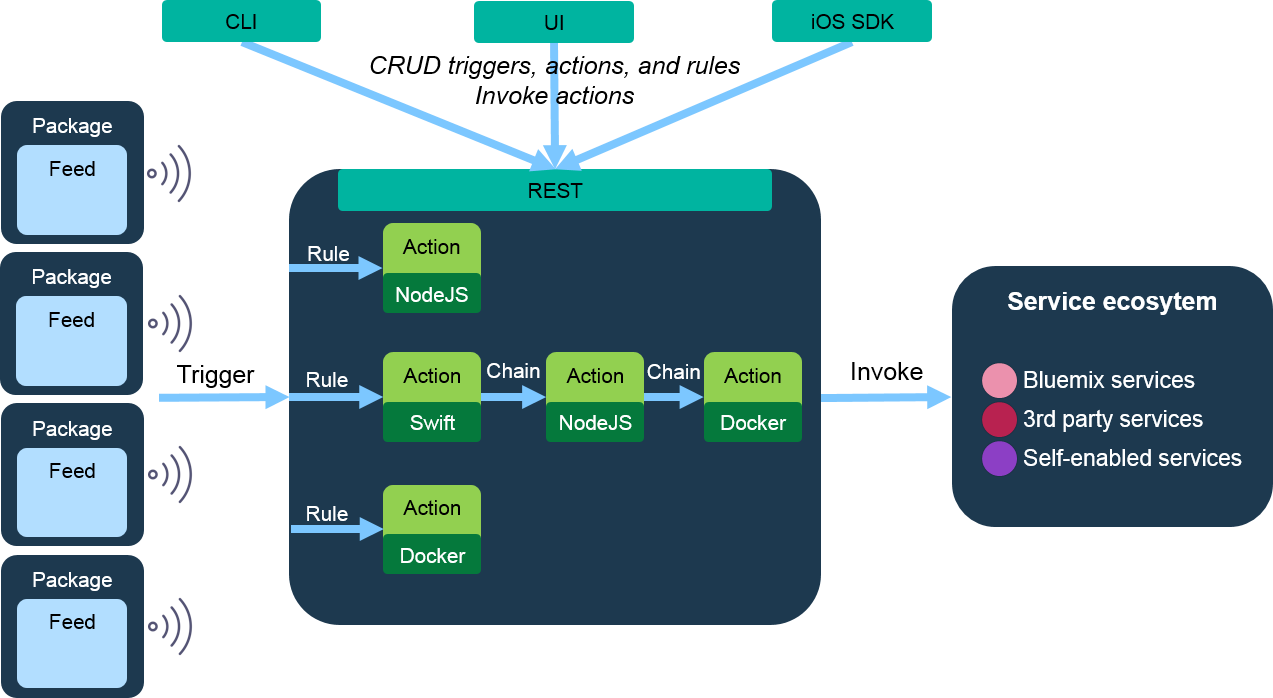
\includegraphics[scale=0.6]{./OpenWhisk}
\caption{OpenWhisk Architecture}
\label{fig:owarch}
\end{figure}
OpenWhisk is a serverless/FaaS platform which executes code in response to events. It supports synchronous, asynchronous and periodic invocation models using an event-driven programming model. Figure \ref{fig:owarch} shows its architecture. Basically, users can store functions or actions in the system that get triggered based on user-specified rules on either periodic events such as alarms or through the exposed REST API from a CLI.

\begin{figure}[htb]
\centering
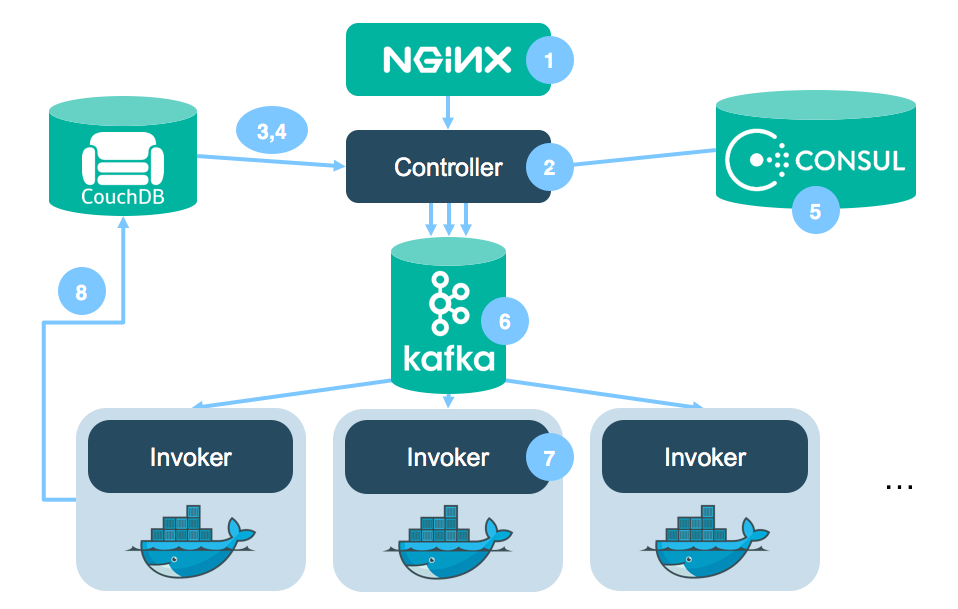
\includegraphics[scale=0.4]{./OpenWhisk_flow_of_processing}
\caption{Internal flow of processing in OpenWhisk}
\label{fig:owflow}
\end{figure}

Figure \ref{fig:owflow} shows what happens inside OpenWhisk during request processing. The system consists of nginx (written in C) for handling HTTP API requests, CouchDB (Erlang) for persistence, Consul (Go) for service discovery, Kafka (Scala, Java) for message queuing (these are all off-the-shelf third-party components), and two custom components written in Scala: a Controller and an Invoker.

When an HTTP request to process an action comes to the system, it is passed by nginx to the Controller (1, 2), which then talks to CouchDB to confirm whether the request can be authenticated and authorized (3). The Controller then retrieves the action associated with the request also stored in CouchDB (4) and then consults Consul to find out which Invoker (executor) is available (5). The Controller then queues the request in Kafka (6) which returns an \emph{ActivationId} that can be returned to the user (in case of an asynchronous request). The Invokers live in sandboxed Docker containers and execute (invoke) the action associated with the request (7). The result is then store in CouchDB (8) to be later retrieved by the user using a similar HTTP request.

\section{Challenges}

The challenges involved in instrumenting such a system are pretty much the same as those described earlier in section \ref{sec:challenge}.

Specifically, we are working on implementing opaque baggage contexts provided by the tracing plane in each component of OpenWhisk: Controller, Invoker, Nginx, CouchDB, Consul and Kafka. It is relatively easy to do that for the Controller and Invoker as both of them are written in Scala and relatively small code bases. Kafka, also written in Scala/Java, should also be easier. But for other components, written in non-JVM languages: C, Erlang and Go, we are limited by the current implementation of Tracing Plane which only supports JVM languages.

An additional challenge is investigating how should invokation models such as asynchronous and periodic requests be supported and exposed to the end user.

\section{Current Status}
We have started out by focusing on the Controller and Invoker which are core parts of OpenWhisk system and the easiest to instrument (among other components). This is reasonable because we can consider serializing and deserializing our baggage contexts into JSON and HTTP headers as part of the usual interactions across system boundaries which should still give us a good picture.

We have successfully integrated\cite[our implementation]{web:instru} Brown Tracing Framework's\cite{web:btf} X-Trace logging on the top of OpenWhisk's custom logging implementation which gives us an initial but partial view of the flow of a client request being processed by OpenWhisk. We are currently in process of integrating more pervasive logging with the help of X-Trace's automatic instrumentation libraries (which are based on AspectJ aspects), which can automatically propagate baggage with each use of Scala's Futures and Promises. This should give us a lot more visibility into the operations of the Controller and the Invokers as they process a request. However, much of the hard work of making rest of the system components interoperate with our baggage remains.

\input{./future-work.tex}
\chapter{Conclusion and Future Work}

We have learned a good deal about the new serverless architecture of computation and specifically, OpenWhisk, during the course of this project. Further, we have learned that distributed tracing is hard on its own even when each system component is locally available; serverless architecture adds another layer of difficulty with the cloud abstraction. Generic opaque baggage contexts proposed in Tracing Plane work can help with the problem of distributed instrumentation for any system. They still require source code modification for each component, however, it needs to be done only once. Tracing plane's layered architecture helps control complexity related to different concerns of developers and hiding subtle details about metadata propagation such as merges and joins across thread, application and machine boundaries. Execution-flow scoped variables built on top of opaque baggage contexts allow different kinds of tracing tools to be implemented much more easily.

In the beginning of the project, we also learned about Conflict-free Replicated Data Types (CRDTs)\cite{Shapiro:2011:CRD:2050613.2050642} which are used in the tracing plane to implement tracing plane BDL (Baggage Definition Language) data types such as flags, counters, sets and maps.

In future, apart from finishing intrumenting OpenWhisk, we would like to port the current tracing plane implementation to support many more languages and runtimes such as Go, Erlang, C/C++ and Rust. We would also like to expand the BDL data type library with more existing CRDTs\cite{shapiro:inria-00555588}.

\cleardoublepage
%\pagebreak
\phantomsection
\addcontentsline{toc}{chapter}{Acknowledgements}
\chapter*{Acknowledgments}
\vspace{0.5in}
I am extremely grateful to my collaborator Jonathan Mace for his continuous guidance and technical help during the course of this work. I am also thankful to Prof. Rodrigo Fonseca for introducing me to this problem and brainstorming initial ideas to approach it.
\vspace{0.5in}

Kartik Singhal
\vspace{0.2in}

May 2017

Brown University

\newpage

\cleardoublepage
\phantomsection
\addcontentsline{toc}{chapter}{References}

\bibliographystyle{acm}
\bibliography{references}


\end{document}
